\chapter{Variables Aleatorias}
Una variable aleatoria $x$ (desde ahora denotada por \textbf{v.a.}) es una función definida sobre el espacio muestral $S$ con valores en $\mathbb{R}$ que a cada elemento de $S$ (Punto muestral) hace corresponder un número real $x=X$.

$$x=X(w) \in Rec_X \subseteq \mathbb{R}$$ 
\subsubsection{Gráficamente}

\begin{center}
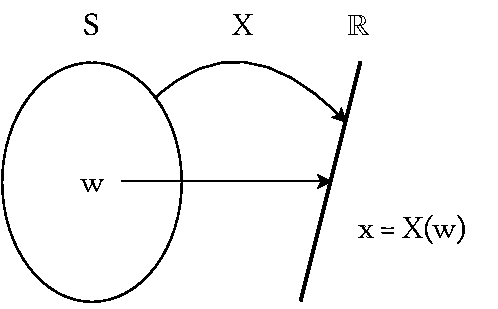
\includegraphics[scale=0.75]{cap1.pdf}
\end{center}

\subsubsection{Notación Conjuntista}
$$X = \lbrace (w,x)\ w\in S, x=X(w)\in \mathbb{R} \rbrace \subseteq S\times  \mathbb{R}$$
Donde:
\begin{itemize}
\item $S$: Conjunto Partida (Espacio Muestral).
\item $\mathbb{R}$: Conjunto de llegada.
\item $w$: Elemento de $S$ (Punto Muestral).
\item $x$: Valor de la \textbf{v.a.} $X$.
\item $Rec_X$: Recorrido de $X$.
\item $X$: Función \textbf{v.a.} (Conjunto de Pares Ordenados).
\end{itemize}
\subsubsection{Notaciones}
Las \textbf{v.a.} se denotan con letras mayúsculas tales como $X,Y$ o $Z$, y los valores correspondientes con letras minúsculas.
\section{Clasificación de Variables Aleatorias}
\begin{itemize}
\item \textbf{Discreta:} Cuyo recorrido es un conjunto finito o infinito numerable de valores:
$$
X \text{ es \textbf{v.a.} discreta} \Rightarrow
\begin{cases}
\text{Conjunto Finito de Valores} \\
\text{Conjunto Infinito Numerable de Valores}
\end{cases}
$$
\item \textbf{Contínua:} Es aquella cuyo recorrido es conjunto finito no numerable de valores, puede tomar cualquier valor en un intervalo o conjunto.
\end{itemize}
$\blacklozenge$ En general las \textbf{v.a.} \textit{discretas} representan datos que provienen del \textit{conteo} de número de elementos. Pueden ser número de titulados, número de estudiantes, etc. Mientras que las \textbf{v.a.} \textit{contínuas} representan mediciones, como longitud, capacidad,etc.
\section{Función de Probabilidad de una Variable Aleatoria}
\noindent También llamada función de cuantía o función de masa de probabilidad de una \textbf{v.a.}. \\${ }$\\
Se denomina función de probabilidad de una \textbf{v.a.} discreta $X$ a una función $p$ o $f$, cuyo valor es $p(x)$ o $P(X=x)0$ ya que a cada valor distinto de la \textbf{v.a.} discreta $X$ hace corresponder en un número entre los valores $[0,1]$ que es su probabilidad, de ahí el nombre de función de cuantía o función de probabilidad. Estos valores satisfacen las siguientes condiciones:
\begin{enumerate}
\item $P(x)\geq 0 \hspace{0.25cm};\hspace{0.25cm} \forall x\in \mathbb{R}$
\item $\displaystyle\sum_{x_i\in Rec_X}^{}p(x_i)=1$
\begin{itemize}
\item Si $Rec_X=\lbrace x_1,x_2,\ldots ,x_n \rbrace$ entonces la condición \textbf{(II)} es: $\displaystyle\sum_{i=1}^{n}p(x_i)=1$
\item Si $Rec_X=\lbrace x_1,x_2,\ldots ,x_n,\ldots \rbrace$ entonces la condición \textbf{(II)} es: $\displaystyle\sum_{i=1}^{\infty}p(x_i)=1$
\end{itemize}
\end{enumerate}
Si $A$ es un evento en el recorrido de la \textbf{v.a.} discreta $X$ entonces la probabilidad de $A$ es el número:
$$P(A)=\displaystyle\sum P(X=x)=\sum p(x)$$
\textbf{Nota:}
$$P(X=x)
\begin{cases}
p(x)\geq 0 ;\hspace{0.25cm} \forall x\in \mathbb{R} \\
f(x)\geq 0 ;\hspace{0.25cm} \forall x\in \mathbb{R}
\end{cases}
$$
La función de probabilidad de una \textbf{v.a.} discreta $X$ se puede expresar por:
\begin{itemize}
\item \textbf{Un Conjunto:} 
$$p=\lbrace (x,P(X))/x\in D_p \rbrace$$
\item \textbf{Una Tabla:}
\begin{center}
\begin{tabular}{|c|c|c|c|c|}
\hline 
$x_i$ & $x_1$ & $x_2$ & $\ldots$ & $x_n$ \\ 
\hline 
$p(x_i)$ & $p(x_1)$ & $p(x_2)$ & $\ldots$ & $p(x_n)$ \\ 
\hline 
\end{tabular} 
\end{center}
\item \textbf{Una Gráfica:}

\begin{center}
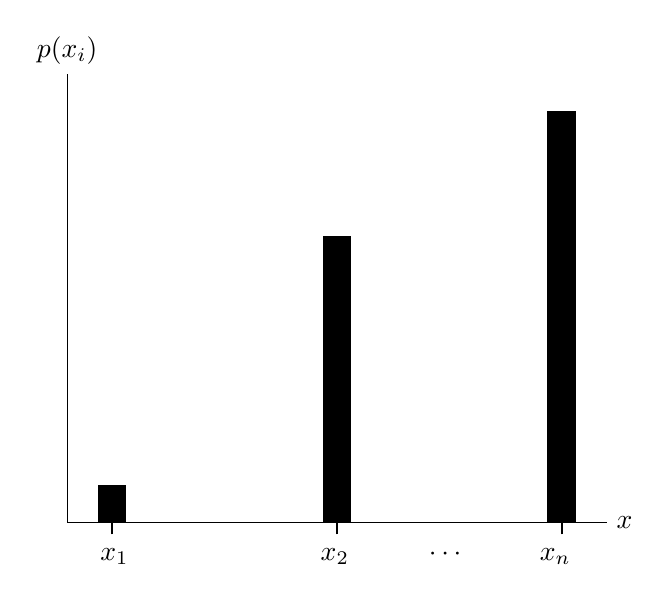
\begin{tikzpicture}

\begin{axis}[
    ybar=15,            
    %ymin=0,
    %ymax=120,            
    symbolic x coords={$x_1$,$x_2$,$x_3$},
    xtick=data,
    yticklabels={,,},
  xticklabels={,,},
  axis lines*=left, xlabel=$x$, ylabel=$p(x_i)$,
  every axis y label/.style={at=(current axis.north west),anchor=south},
  every axis x label/.style={at=(current axis.right of origin),anchor=west},
  ytick=\empty,
  major tick style = {thick, black}]
  
  \addplot[ybar,fill=black] coordinates {
                ($x_1$,   50)
                ($x_2$,  70)
                ($x_3$,   80)
            };
\end{axis}

\node[below] at (0.6,-0.2)  {$x_1$}; 
\node[below] at (3.4,-0.2)  {$x_2$}; 
\node[below] at (4.8,-0.2)  {$\cdots$}; 
\node[below] at (6.2,-0.2)  {$x_n$}; 


\end{tikzpicture}
\end{center}

\end{itemize}
\section{Función de Distribución Acumulada (FDA)}
El valor de la \textbf{FDA} de una \textbf{v.a.} discreta $X$, que es $F(x)$, viene dada por la sumatoria de las probabilidades, desde un valor mínimo $t$ hasta un valor específico $x$; esto es:
$$F(x)=P(X\leq x)=\displaystyle\sum_{t\leq x} P(t),\hspace{0.25cm} \forall x\in \mathbb{R}$$
\subsection{Representación Gráfica}
Valores $F(x)$ aumentan en \textit{saltos}, presentando entonces la forma de una escalera:
\begin{center}
\begin{tikzpicture}[
    declare function={gamma(\z)=
    2.506628274631*sqrt(1/\z)+ 0.20888568*(1/\z)^(1.5)+ 0.00870357*(1/\z)^(2.5)- (174.2106599*(1/\z)^(3.5))/25920- (715.6423511*(1/\z)^(4.5))/1244160)*exp((-ln(1/\z)-1)*\z;},
    declare function={gammapdf(\x,\k,\theta) = 1/(\theta^\k)*1/(gamma(\k))*\x^(\k-1)*exp(-\x/\theta);}
]

\begin{axis}[
  no markers, domain=0:4, samples=300,
  axis lines*=left, xlabel=$x$, ylabel=$F(x)$,
  every axis y label/.style={at=(current axis.above origin),anchor=south},
  every axis x label/.style={at=(current axis.right of origin),anchor=west},
  height=5cm, width=8cm,
  yticklabels={,,},
  xticklabels={,,},
  enlargelimits=false, clip=false, axis on top,
    ytick=\empty,
  xtick=\empty,
  major tick style = {thick, white}
  ]
\end{axis}

\node[below] at (1,-0.1)  {$x_1$}; 
\node[below] at (2,-0.1)  {$x_2$}; 
\node[below] at (3,-0.1)  {$x_3$}; 
\node[below] at (4,-0.1)  {$\cdots$}; 

\node[left] at (0,1)  {$F(x_1)$}; 
\node[left] at (0,2)  {$F(x_2)$}; 
\node[left] at (0,3)  {$F(x_3)$}; 

\draw [very thick,dotted, line width=0.4mm]  (1,0) -- (1,1);
\draw [very thick,dotted, line width=0.4mm]  (2,1) -- (2,2);
\draw [very thick,dotted, line width=0.4mm]  (3,2) -- (3,3);
\draw [very thick,dotted, line width=0.4mm]  (4,3) -- (4,4);

\draw [very thick, line width=0.4mm]  (0,0) -- (1,0);
\draw [very thick, line width=0.4mm]  (1,1) -- (2,1);
\draw [very thick, line width=0.4mm]  (2,2) -- (3,2);
\draw [very thick, line width=0.4mm]  (3,3) -- (4,3);

\node[] at (1,1) {$\bullet$}; 
\node[] at (2,2)  {$\bullet$}; 
\node[] at (3,3)  {$\bullet$}; 

\node[circle,fill=white, draw=black!80, thick, inner sep=0pt, minimum size=6pt] (1) at (1,0) {};
\node[circle,fill=white, draw=black!80, thick, inner sep=0pt, minimum size=6pt] (1) at (2,1) {};
\node[circle,fill=white, draw=black!80, thick, inner sep=0pt, minimum size=6pt] (1) at (3,2) {};

\end{tikzpicture}
\end{center}
\subsection{Caso Continuo}
\subsubsection{Función de Densidad}
$f$ es función densidad, si $f(x)$ cumple las siguientes condiciones:
\begin{enumerate}[label=(\roman*)]
\item $f(x)\geq 0;\hspace{0.25cm} \forall x\in \mathbb{R}$
\item $\displaystyle\int_{-\infty}^{\infty}f(x) dx = 1$
\item $p(a\leq x \leq b)=\displaystyle\int_{a}^{b}f(x)dx$
\end{enumerate}
\subsubsection{FDA}
$$F(x)=P(X\leq x)=\displaystyle\int_{-\infty}^{x} f(x) dx$$
\subsection{Propiedades de la FDA}
\subsubsection{Caso Discreto}
\begin{enumerate}
\item $0\leq F(x) \leq 1;\hspace{0.25cm}\forall x\in\mathbb{R}$
\item $F(-\infty)=0$
\item $F(+\infty)=1$
\item $P(X\leq a) = F(a)$
\item $P(X>a)=1-P(X<a)=1-F(a)$
\item $P(X<a)=
\begin{cases}
F(a-1), \text{si } a\in\mathbb{Z} \\
F([\![ a ]\!]), \text{si } a\notin \mathbb{Z}
\end{cases}
$
\item $P(X\leq -a)=1-P(X\leq a)=1-F(a)$
\item $P(a<X\leq b)=F(b)-F(a)$
\item $P(a\leq X \leq b)=F(b)-F(a)+P(X=x)$
\item $P(a<X<b)=F(b)-F(a)-P(X=b)$
\item $P(X=x_i)=F(x_i)-F(x_{i-1})$
\end{enumerate}
\subsubsection{Caso Continuo}
\begin{enumerate}
\item $0\leq F(x) \leq 1; \hspace{0.25cm}\forall x\in\mathbb{R}$
\item $F(-\infty)=0$
\item $F(+\infty)=1$
\item $P(X\leq a)=P(X<a)=F(a)$
\item $P(X>a)=1-P(X\leq a)=1-F(a)$
\item $P(X\geq a)=1-P(X<a)=1-F(a)$
\item $P(X\leq -a)=1-P(X\leq a)=1-F(a)$
\item $P(a<X\leq b)=P(a\leq X\leq b)=P(a<X<b)$
\item $f(x)=\dfrac{d F(x)}{dx}$
\end{enumerate}
\section{Esperanza Matemática}
Sea $X$ una \textbf{v.a.} con función de probabilidad $f$ definida por $f(x)$. La \textit{esperanza matemática} de $X$, denotada por $E(x),\mu$ ó $\mu_x$; está dada por:

$$
E(x)=\mu =\mu_x =
\begin{cases}
\displaystyle\sum_{x} x\cdot p(x), \text{ Si $X$ es \textbf{v.a.} Discreta}\vspace{0.25cm}\\
\displaystyle\int_{-\infty}^{+\infty} x\cdot f(x) dx, \text{ Si $X$ es \textbf{v.a.} Continua}
\end{cases}
$$
\subsubsection{Propiedades}
\begin{enumerate}
\item $E(a)=a$
\item $E(x\pm a)=E(x)\pm a$
\item $E(ax)=aE(x)$
\item $E(ax\pm b)=aE(x)\pm b$
\end{enumerate}
\subsection{Varianza}
Notaciones: $V(x),\sigma^2,\sigma_{x}^{2}$
$$
V(x)=\sigma^2 =
\begin{cases}
E[x-\mu]^2 = \displaystyle\sum_{x} (x-\mu)^2 f(x); \text{ Si $X$ es \textbf{v.a.} Discreta}\vspace{0.25cm}\\
E[x-\mu]^2 = \displaystyle\int_{-\infty}^{+\infty} (x-\mu)^2 f(x)dx; \text{Si $X$ es \textbf{v.a.} Continua}
\end{cases}
$$
\subsubsection{Propiedades}
\begin{enumerate}
\item $V(x)\geq 0$
\item $V(a)=0$
\item $V(ax)=aV(x)$
\item $V(ax\pm b)=a^2 V(x)$
\item $V(x)=E(x^2)-[E(x)]^2$
\end{enumerate}
\begin{multicols}{2}
\begin{flushleft}
\end{flushleft}
\columnbreak
\end{multicols}
\section{Función de Probabilidad Conjunta}
\subsection{Función de Cuantía Conjunta}
$$P(X=x,Y=y)=f(x,y)=p(x,y)$$
es el valor de una función de cuantía conjunta de la \textbf{v.a.'s} $X$ y $Y$ si:
\begin{enumerate}[label=(\roman*)]
\item $f(x,y)=p(x,y)\geq 0$ \hspace{2cm} Para cualquier $(x,y)$ de su dominio.
\item $\displaystyle\sum_{x}\displaystyle\sum_{y} f(x,y)=1$
\item $P((x,y)\in A)=\displaystyle\sum _A\displaystyle\sum f(x,y)$ \hspace{2cm} Para cualquier región $A$ del plano $XY$.
\end{enumerate}
\subsection{Función de Densidad Conjunta}
$$P(X=x,Y=y)=f(x,y)=p(x,y)$$
es el valor de una función de cuantía conjunta de la \textbf{v.a.'s} $X$ y $Y$ si:
\begin{enumerate}[label=(\roman*)]
\item $f(x,y)=p(x,y)\geq 0$ \hspace{2cm} Para cualquier $(x,y)$ de su dominio.
\item $\int\limits_{-\infty}^{+\infty} \int\limits_{-\infty}^{+\infty} f(x,y) \,dx \,dy=1$
\item $P((x,y)\in A)=\iint_A f(x,y) \,dx \,dy$ \hspace{2cm} Para cualquier región $A$ del plano $XY$.
\end{enumerate}
\section{Distribuciones Marginales}
Sean $X$ y $Y$ \textbf{v.a.} con función de probabilidad conjunta definida por $f(x,y)$. La distribución marginal está dada por:
$$
\text{Caso Discreto:}
\begin{cases}
\text{Distribución Marginal X: } g(x)=\displaystyle\sum_{y}f(x,y)  \\ \vspace{0.1cm} \\
\text{Distribución Marginal Y: } h(y)=\displaystyle\sum_{x}f(x,y)
\end{cases}
$$
$$
\text{Caso Continuo:}
\begin{cases}
\text{Distribución Marginal X: } g(x)=\displaystyle\int_{-\infty}^{+\infty} f(x,y) \,dy \\ \vspace{0.1cm} \\
\text{Distribución Marginal Y: } h(y)=\displaystyle\int_{-\infty}^{+\infty} f(x,y) \,dx
\end{cases}
$$
\subsection{Independencia Estadística de las v.a. $X$ y $Y$}
Sean $X$ y $Y$ \textbf{v.a.} discretas o contínuas con función de probabilidad conjunta definida por $f(x,y)$ y distribuciones marginales $g(x)$ y $h(y)$, respectivamente. Se dice que las \textbf{v.a.} $X$ y $Y$ serán estadísticamente independientes ssi:

$$f(x,y)=g(x)h(y)$$
Para cualquier $(x,y)$ dentro de sus recorridos.
\subsection{Esperanza Matemática}
Sean $X$ y $Y$ \textbf{v.a.} con función de probabilidad definida por $f(x,y)$. La media o esperanza matemática de $g(x,y)$ está dada por:
$$
\text{Caso Discreto: }
E(g(x,y))=\mu_{g(x,y)}=\displaystyle\sum_{x}\displaystyle\sum_{y} g(x,y)\cdot f(x,y)
$$

$$
\text{Caso Contínuo: }
E(g(x,y))=\mu_{g(x,y)}=\displaystyle\int_{-\infty}^{+\infty}\displaystyle\int_{-\infty}^{+\infty} g(x,y)\cdot f(x,y) \,dx \,dy
$$
\subsection{Covarianza}
Mide el grado de relación o asociación de dos variables.
\subsection{Resultado Importantes}
\begin{enumerate}
\item $E(x\pm y)=E(x)\pm E(y)$
\item $Cov(x,y)=E(x\cdot y) - E(x)E(y)$
\item $V(x\pm y)=V(x)+V(y)\pm 2Cov(x,y)$
\item $V(ax\pm by)=a^2 V(x)+b^2V(y)\pm 2abCov(x,y)$
\item Si $X$ y $Y$ son estadísticamente independientes entonces:
\begin{enumerate}
\item $E(x,y)=E(x)E(y)$
\item $Cov(x,y)=0$
\item $V(x\pm y)=V(x)+V(y)$
\item $V(ax\pm by)=a^2V(x)+b^2V(y)$

\end{enumerate}
\item Si $x1,x2,x3,\ldots$ son variables aleatorias independientes 2 a 2:\\ \vspace{0.025cm} \\
$V\Bigg( \displaystyle\sum_{i=1}^{m} x_i \Bigg) = \displaystyle\sum_{i=1}^{m} V(x_i)$
\end{enumerate}